\chapter{Ubicar a la persona: localización y fusión}
\label{cap:localizacion}

\begin{enpocas}
Cómo se convierte un recuadro de la imagen en un punto del suelo, de dónde viene el error y cómo se
calcula su tamaño (propagación de covarianza), y cómo se juntan muchas detecciones de la misma persona
en una sola candidata cada vez más precisa y confiable.
\end{enpocas}

\section{Del recuadro al suelo: el rayo}

Para cada detección se toma el centro del recuadro $(u,v)$ ---con la cámara hacia abajo, la persona se
ve casi desde arriba y el centro es el mejor punto de apoyo---. Su dirección en el marco de la cámara es
$K^{-1}(u, v, 1)^\top$; se pasa al mundo con la orientación de la cámara ($R_{BC}$, fija respecto al
cuerpo) y la del dron ($R$, que estima PX4):
\begin{equation}
r = R\,R_{BC}\,K^{-1}\begin{bmatrix}u\\v\\1\end{bmatrix},\qquad p_c = \xi + R\,t_{BC},
\end{equation}
donde $\xi$ es la posición del dron y $t_{BC} = (0, 0, -0.25)$~m la de la cámara (bajo los patines).
El punto del suelo ($z = z_t = 0$) es
\begin{equation}
x = p_c + \lambda\,r,\qquad \lambda = \frac{z_t - p_{c,z}}{r_z}.
\end{equation}
Si el rayo no baja ($r_z \ge 0$) no hay intersección; si forma más de 60° con la vertical, el error
sería enorme y se descarta (ver el recuadro de abajo).

\begin{figure}[H]
\centering
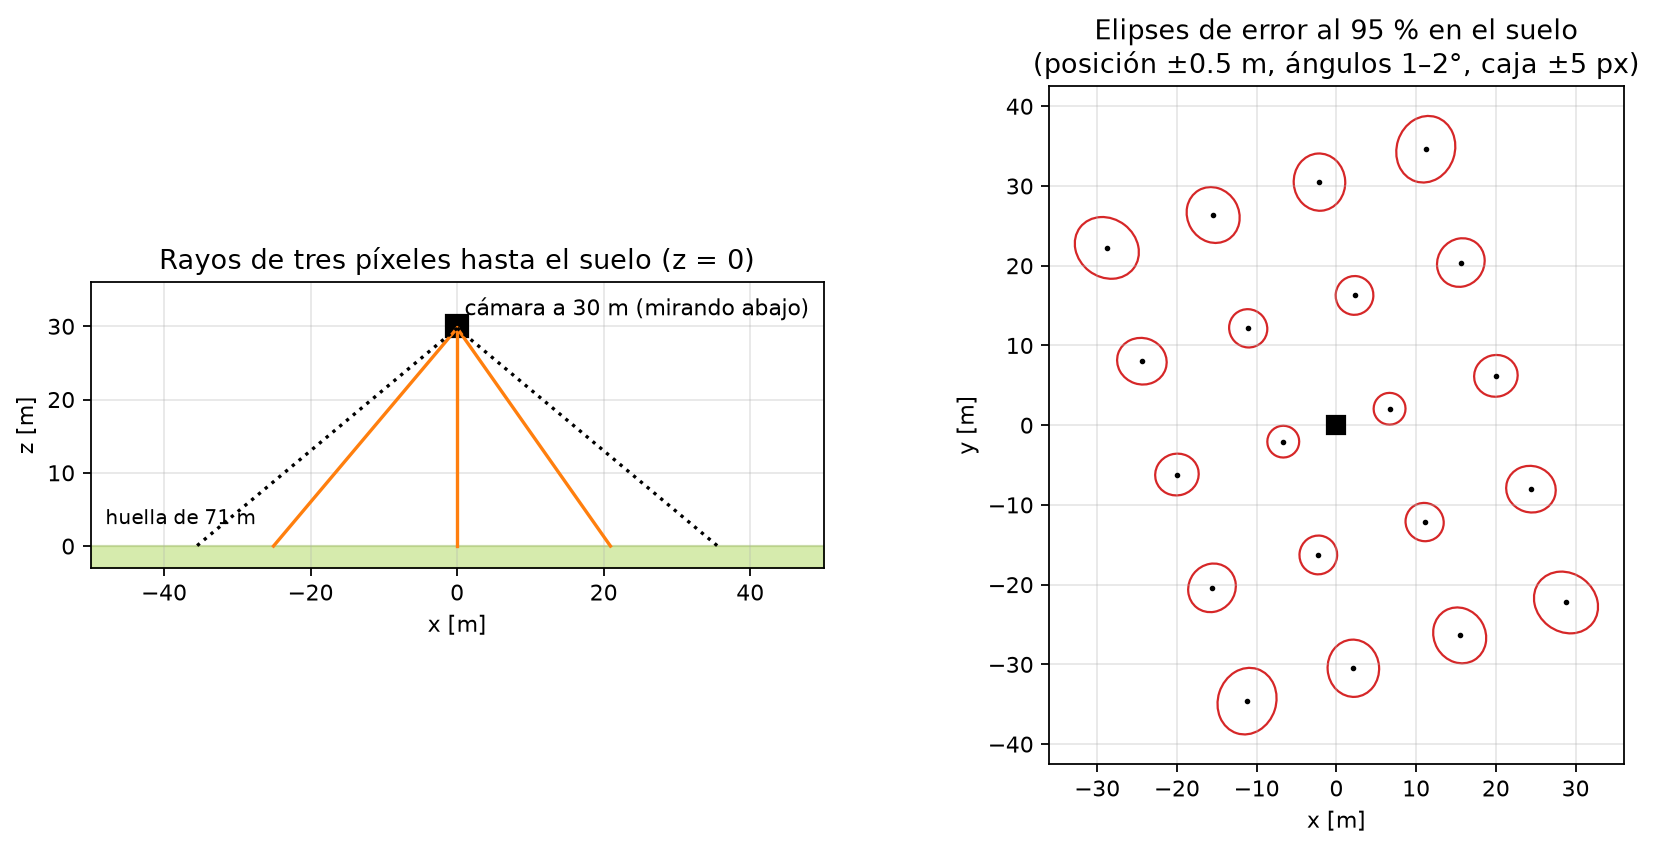
\includegraphics[width=\textwidth]{localizacion.png}
\caption{Izquierda: rayos de tres píxeles hasta el suelo. Derecha: elipses de error al 95~\% para una
rejilla de píxeles, con la incertidumbre típica de PX4.}
\label{fig:localizacion}
\end{figure}

\section{¿Qué tan grande es el error?}

El punto depende de ocho cantidades inciertas: la posición del dron (3), su orientación (3) y el
centro del recuadro (2). Si cada una tiene una varianza conocida ($\Sigma_p$, $\Sigma_\eta$, $\Sigma_u$),
a primer orden la covarianza del punto es
\begin{equation}
\Sigma_x \approx J_p\Sigma_pJ_p^\top + J_\eta\Sigma_\eta J_\eta^\top + J_u\Sigma_uJ_u^\top ,
\end{equation}
con $J$ las derivadas (jacobianos) de $x$ respecto a cada grupo, calculadas numéricamente. La elipse de
la figura~\ref{fig:localizacion} es la representación de $\Sigma_x$. PX4 publica las varianzas de su
estimación en \cod{/fmu/out/vehicle_odometry}, así que el localizador las usa en cada detección.

\begin{ejemplo}
Apuntar con un láser desde un balcón: un pequeño temblor de la mano (orientación) mueve el punto más
cuanto más lejos está el suelo; moverse uno mismo medio metro (posición) mueve el punto medio metro,
esté donde esté. Por eso el error por orientación crece con la altura y el de posición no.
\end{ejemplo}

\cod{codigo/sim_localizacion.py} valida la fórmula con miles de simulaciones al azar (Monte Carlo) y
separa las tres fuentes:

\begin{table}[H]
\centering\small
\begin{tabular}{lccccc}
\toprule
\textbf{Caso} & \textbf{altura} & \textbf{RMSE Monte Carlo} & \textbf{por posición} & \textbf{por orientación} & \textbf{por detección} \\ \midrule
nominal ($\sigma_p$ = 0.5 m, $\sigma_\eta$ = 0.5°, $\sigma_u$ = 5 px) & 20 m & 0.85 m & 0.92 & 0.31 & 0.26 \\
nominal & 30 m & 0.94 m & 0.92 & 0.47 & 0.39 \\
nominal & 40 m & 1.05 m & 0.92 & 0.62 & 0.52 \\
posición degradada ($\sigma_p$ = 2 m) & 30 m & 3.02 m & 3.34 & 0.47 & 0.39 \\
orientación degradada ($\sigma_\eta$ = 2°) & 30 m & 1.81 m & 0.92 & 1.86 & 0.39 \\
detección degradada ($\sigma_u$ = 20 px) & 30 m & 1.78 m & 0.92 & 0.47 & 1.57 \\
\bottomrule
\end{tabular}
\caption{Error de localización y su desglose (salida de \cod{sim_localizacion.py}; las tres últimas
columnas son la contribución lineal en metros). Con un GPS normal domina la posición del dron.}
\end{table}

\begin{figure}[H]
\centering
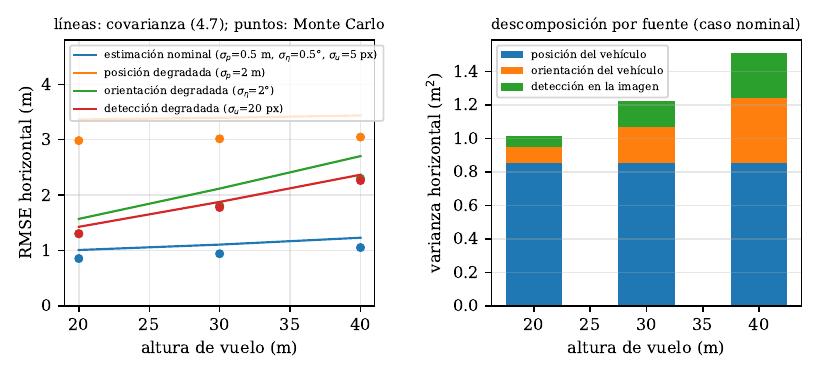
\includegraphics[width=0.85\textwidth]{manual_sim_localizacion.png}
\caption{Figura de \cod{sim_localizacion.py}: la fórmula lineal y el Monte Carlo coinciden.}
\end{figure}

\section{Juntar detecciones: asociación y fusión}

A 3~m/s, una persona queda en la imagen varios segundos y el detector la ve decenas de veces. Cada
detección produce un punto con su elipse. \cod{localizador_node} mantiene una lista de
\textbf{candidatas} y, para cada detección nueva:
\begin{enumerate}
  \item \textbf{Asociación:} calcula su distancia de \textbf{Mahalanobis} a cada candidata,
        \begin{equation}
        d^2 = (x - c)^\top(\Sigma_x + \Sigma_c)^{-1}(x - c),
        \end{equation}
        una distancia ``medida en elipses''. Si la menor es menor que 9.21 (el percentil 99~\% de una
        $\chi^2$ con 2 grados de libertad), es la misma persona; si no, nace una candidata nueva.
  \item \textbf{Fusión:} combina las dos estimaciones pesando cada una por su precisión (fusión de
        información):
        \begin{equation}
        \Sigma_c' = \big(\Sigma_c^{-1} + \Sigma_x^{-1}\big)^{-1},\qquad
        c' = \Sigma_c'\big(\Sigma_c^{-1}c + \Sigma_x^{-1}x\big).
        \end{equation}
        La candidata nueva $c'$ queda más cerca de la estimación más precisa, y su elipse $\Sigma_c'$ es
        siempre más chica que las dos anteriores.
  \item \textbf{Confianza:} acumula la confianza del detector como la probabilidad de que al menos una
        detección sea correcta: $C \leftarrow 1 - (1 - C)(1 - c_i)$.
\end{enumerate}

\begin{figure}[H]
\centering
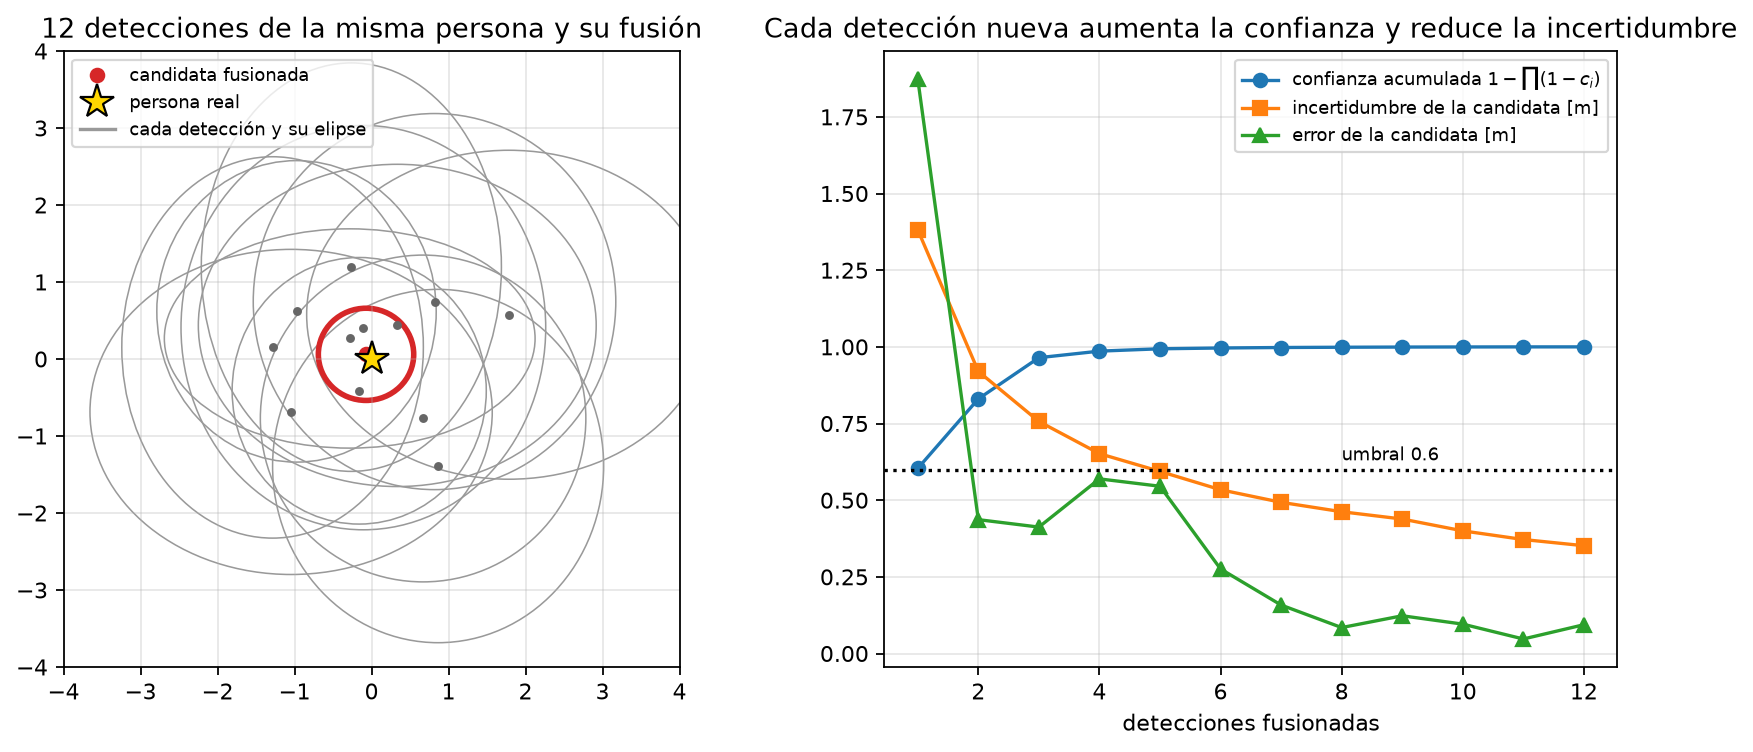
\includegraphics[width=\textwidth]{fusion.png}
\caption{Doce detecciones simuladas de una persona: cada una con su elipse (gris) y la candidata
fusionada (rojo). Con cada detección la confianza sube y la incertidumbre baja.}
\end{figure}

La misión considera \textbf{detectada} a una candidata con confianza acumulada $\ge$ 0.6, y una persona
\textbf{localizada} si alguna detectada queda a menos de 5~m (asignación uno a uno). Las detectadas que
no corresponden a nadie son \textbf{falsas alarmas}.

\begin{leccion}
La confianza acumulada sube muy rápido: dos detecciones de 0.5 ya dan 0.75. Por eso una sombra vista
dos veces ya cuenta como candidata confirmada. En las pruebas, exigir además al menos 10 detecciones
fusionadas bajó las falsas alarmas de 28--31 a 4--5 por vuelo sin perder personas; los avisos GPS usan
ese criterio. Las falsas alarmas que quedan son persistentes: grupos de robles que el detector confunde
una y otra vez.
\end{leccion}

\begin{leccion}
En las vueltas de la ruta el dron se inclina; la cámara, que mira hacia abajo, alcanzaba a ver cerca del
horizonte, y un rayo casi horizontal cortaba el suelo a cientos de metros: salían candidatas a 250~m,
fuera del bosque. El localizador ahora descarta rayos a más de 60° de la vertical (con el dron nivelado
las esquinas de la imagen quedan a $\approx$57°, así que en vuelo normal no se pierde nada).
\end{leccion}

\begin{leccion}
PX4 marca sus mensajes con el reloj de la computadora y la cámara con el de Gazebo. Emparejar cada
imagen con la pose del dron en ese instante exige conocer el desfase; el localizador lo estima con el
mínimo de (llegada $-$ marca) en tiempo simulado.
\end{leccion}
